\chapter{Radioactivité $\alpha$}
\section{Définitions et conservation de l'énergie}
La radioactivité $\alpha$ est définie par la processus suivant
\begin{equation}
^A_ZX \to ^{A-4}_{Z-2}Y + \alpha
\end{equation}
où $X$ est le noyau mère, $Y$ le noyau fille et $\alpha$ est un noyau $^4$He ($Z=N=2$). Supposons que le 
noyau $X$ soit au repos et le noyau $Y$ dans son état fondamental. Par conservation de l'énergie
\begin{equation}
T_Y+T_\alpha = Q_\alpha = (m_X-m_Y-m_\alpha)c^2 > 0
\end{equation}
Pour avoir radioactivité $\alpha$, il faut donc que $m_X > m_Y+m_\alpha$. On peut en déduire les énergies 
cinétiques à partir de la conservation de l'impulsion $\vec{p}_Y+\vec{p}_\alpha=\vec0$. Nous avons $m_YT_Y=
m_\alpha T_\alpha$ et donc
\begin{equation}
T_\alpha = \left(1-\frac{4}{A}\right)Q_\alpha,\qquad\qq T_Y= \frac{4}{A}Q_\alpha
\end{equation}
Il s'agit d'un processus à deux corps impliquant que les particules $\alpha$ soient monocinétiques. 
L'énergie de la transition (énergie libérée) est donc essentiellement portée par la particule $\alpha$. On
appelle $T_Y$ l'\textbf{énergie de recul} du à l’émission, qui est faible (ce qui est le cas en général) si
$A$ est grand.

\section{Conditions de décroissance $\alpha$}
L'idée est toujours la même (et nous avons déjà énoncé cette condition ci-dessus) : la masse initiale doit être
plus grande que la somme des deux masses ($m=Z*m_p+N*m_n-B$). Généralement, on parle d'énergie de liaison et non de
masses
\begin{equation}
\begin{array}{ll}
Q_\alpha &= (m(A,Z)-m(A-4,Z-2)-m(4,2))c^2\\
&= B(4,2)+B(A-4,Z-2)-B(A,Z) >0
\end{array}
\end{equation}
Il faut donc que
\begin{equation}
B(4,2) > A\frac{B(A,Z)}{A}-(A-4)\frac{B(A-4,Z-2)}{A-4}
\end{equation}
En moyenne (la fameuse valeur de 7-8 MeV, il s'agit du rapport $B/A$ moyen).
\begin{equation}
\left(\frac{B(A,Z)}{A}\right)_m < \frac{B(4,2)}{4}\approx 7\text{ MeV}
\end{equation}

\newpage
	\begin{wrapfigure}[10]{r}{6cm}
%	\vspace{-5mm}
	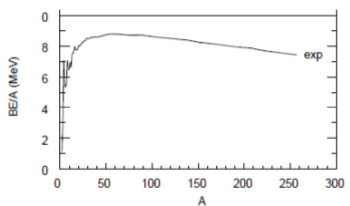
\includegraphics[scale=0.4]{ch5/image1}
	\captionof{figure}{ }
	\end{wrapfigure}

Ce rapport $B/A$ moyen doit être inférieur à l'énergie de la particule $\alpha$ qui est extrêmement liée. En 
regardant la courbe $B/A$, la décroissance $\alpha$ ne peut se produire que pour des noyaux. Si on regarde
la courbe, on pourrait même croire que ça n'arrive jamais mais il ne faut pas oublier que cette courbe correspond
au cas stable : ça arrive donc en pratique. Pourquoi n'y a-t-il pas d'autres radioactivité (comme en deuton)? Car
la particule $\alpha$ est très liée ($B/A$ pour le deuton est de 1.1 MeV) et peut facilement se faire éjectée.


\section{Durée de vie - effet tunnel}
Il n'est pas possible d'utiliser la règle d'or de \textsc{Fermi}, le potentiel n'étant pas petit. On va supposer
une décroissance $X\to Y+\alpha$ où la formation de la particule $\alpha$ se fait à la surface. 
\begin{center}
	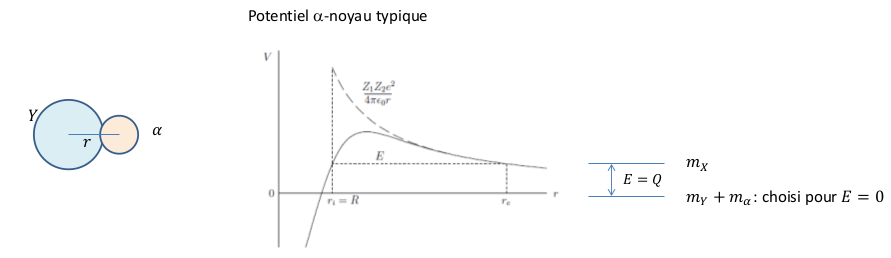
\includegraphics[scale=0.5]{ch5/image2}
	\captionof{figure}{ }
\end{center}
Le potentiel 
est attractif à faible distance (nucléaire) et répulsif à longue distance (Coulomb) : il s'agit des deux cas 
extrêmes qui sont "relié" par la \textit{barrière de potentiel}. Cette barrière de potentiel doit être franchie
pour avoir émission d'une particule $\alpha$ mais ceci ne peut se faire que par effet tunnel (impossible donc dans
un cas classique). Si le seuil est trop petit, la probabilité peut être suffisamment petite pour que la durée de
vie soit énorme : il est nécessaire de calculer le \textbf{coefficient de transmission} qui sera proportionnel
à la probabilité de désintégration.\\

	\begin{wrapfigure}[6]{r}{6cm}
	\vspace{-8mm}
	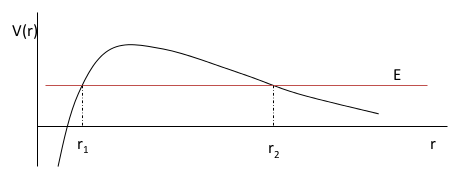
\includegraphics[scale=0.4]{ch5/image3}
	\captionof{figure}{ }
	\end{wrapfigure}

Le calcul de ce coefficient se fait grâce à l'approximation \textsc{WKB} : on résout l'approximation 
$u''(r)-\frac{2\mu}{\hbar^2}(V(r)-E)u(r)=0$ en posant $u(r) = \exp(iS(r))$ ($S(r)$ varie lentement) et on en 
déduit $S(r)^{'2} = \frac{2\mu}{\hbar^2}(E-V(r))$. En remplaçant dans l'équation de \textsc{Schrödinger}, on 
en déduit (si $E<V(r)$)
\begin{equation}
u(r) = \exp\left(-\int_0^r \sqrt{\frac{2\mu}{\hbar^2}(V(r)-E)}\text{d}r\right)
\end{equation}
Ce qui nous intéresse n'est pas l'amplitude de la fonction d'onde mais le coefficient de transmission $T$. 
Celui-ci n'est rien d'autre que la probabilité d'être en $r_2$ sur la probabilité d'être en $r_1$ 
\begin{equation}
T = \left|\dfrac{u(r_2)}{u(r_1)}\right|^1 = \exp\left( -2\int_{r_1}^{r_2} \sqrt{\frac{2\mu}{\hbar^2}(V(r)-E)}
\text{d}r\right)
\end{equation}
En remplaçant l'expression de $V(r)$, il est souvent impossible d'obtenir une solution analytique mais bien
numérique (simple calcul d'intégral).\\


	\begin{wrapfigure}[9]{r}{4.5cm}
	\vspace{-5mm}
	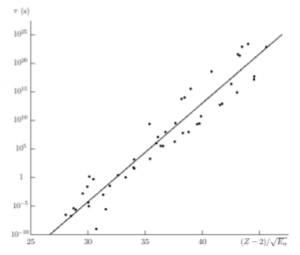
\includegraphics[scale=0.4]{ch5/image4}
	\captionof{figure}{ }
	\end{wrapfigure}
	
Pour un potentiel purement coulombien ($m=0$): $r_1=R, r_2=\frac{Z_1Z_2e^2}{E}$ avec $Z_2=2, Z_1=Z-2$, on 
trouve
\begin{equation}
T \approx \exp(-2\pi\eta)
\end{equation}
où $\eta= Z_1Z_2\alpha(c/v) : Z_1Z_2\alpha\sqrt{(2\mu c^2)/E}$ est le paramètre de \textsc{Sommerfeld} (où
$\alpha = 1/137$). Si l'énergie diminue, $\eta$ augmente et donc $T$ diminue. Cette propriété se retrouve
dans la durée de vie ($\tau$ augmente lorsque $E$ diminue : loi de \textsc{Geiger-Nuttall})
La durée de vie $\tau \propto 1/T$ vaut alors
\begin{equation}
\log\tau = C_1+C_2\frac{Z-2}{\sqrt{E}}
\end{equation}
où $C_2 = 2\pi\alpha\sqrt{2\mu c^2}$ (il est possible de retrouve $C_1$ à l'aide de coefficients).
Il y a parfois de très grandes variations, essentiellement parce que notre modèle est très approximatif : il 
ne prend pas en compte la formation de particule $\alpha$ dans le noyau mais le résultat est déjà pas mal.


\section{Conservation du moment cinétique}
Le moment cinétique est défini $\vec{J_X}=\vec{J_Y}+\vec{J_\alpha}+l$ tandis que la parité $\pi_X=\pi_Y\pi_\alpha
(-1)^l$. Pour une particule $\alpha$ : $J_\alpha=0, \pi_\alpha=+1$. Comme en général $J_X=0, \pi_X=+1$, il faut 
que $J_Y=l$.\\

Lorsque $l$ augmente, une barrière centrifuge apparaît. La probabilité de désintégration diminue et il y a un
double effet du moment cinétique $(Q_\alpha,l)$
\begin{equation}
Q_\alpha = (m_X-m_{Y^*}-m_\alpha)c^2
\end{equation}
Le coefficient de transmission $T_l/T_0$ pour $Z=88,l=2$ vaut 0.37, $l=4$ donne 0.037 et $m=6$ donne 0.001, la
tendance est bien vérifiée.\\


\begin{center}
	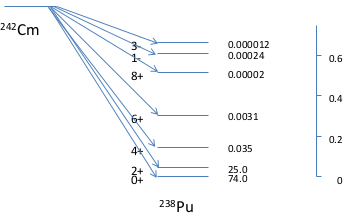
\includegraphics[scale=0.65]{ch5/image5}
	\captionof{figure}{Schéma de désintégration vers le fondamental mais avec une série de niveau toujours en dessous du seuil. La 
transition vers un état excité à deux effets : le zéro des énergies doit être remonté (diminution du seuil, 
cause une diminution de la probabilité de désintégration) et l'effet centrifuge avec $l$ (une augmentation de 
$l$ augmente la barrière) : probabilité de désintégration vers d'autres états beaucoup plus petits.
}
\end{center}